\StartPlate{V10}{A larger inducing carrier can return the same object}{Induction in stages changes the intermediate group without changing the result.}
\begin{center}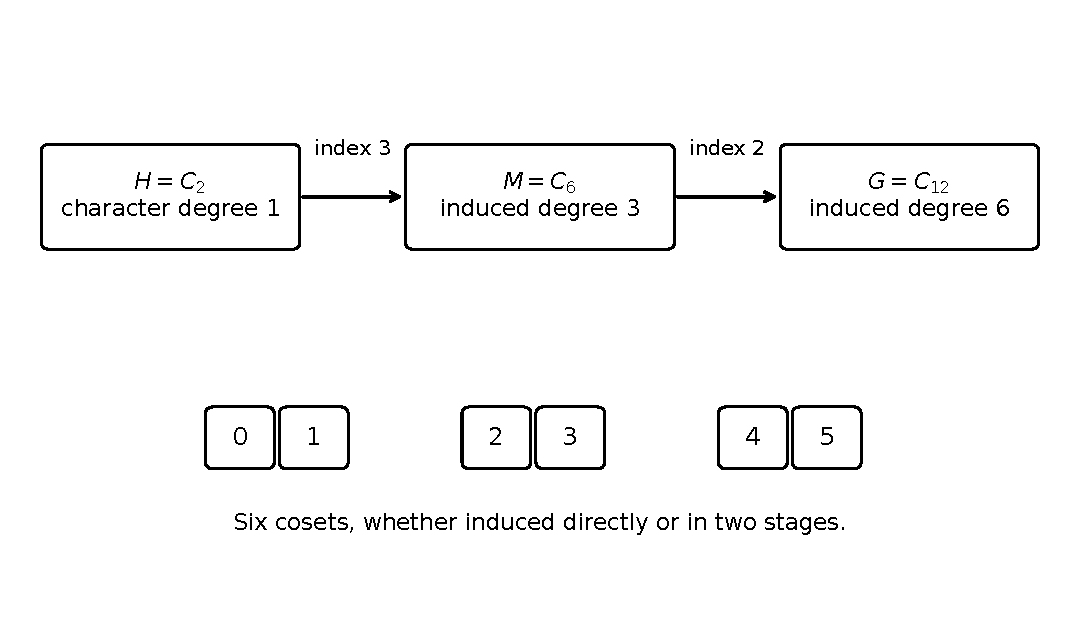
\includegraphics[width=\linewidth]{figures/V10.pdf}\end{center}
The diagram is a finite analogue, not the actual local-field construction. Use $H=C_2\subset M=C_6\subset G=C_{12}$ and a character of $H$. Induction to $M$ has dimension three, and induction onward to $G$ has dimension six. Direct induction has the same six cosets, represented by $i+2j$ with $i\in\{0,1\}$ and $j\in\{0,1,2\}$.
\[
\operatorname{Ind}_M^G\operatorname{Ind}_H^M\lambda
\simeq\operatorname{Ind}_H^G\lambda.
\]
The arithmetic recovery uses the corresponding compact-induction transitivity with the original full inducing representation $\Lambda$. Its larger intermediate carrier must be an actual permitted subgroup, and the original central character and noncompact extension must be retained.

The rank-two and rank-four proofs supply additional group, normalization, and character-orbit arguments before transitivity applies. The finite coset calculation isolates the recovery mechanism. It neither constructs those arithmetic groups nor proves irreducibility of a new local-field representation.
\vfill\PlateSource{Exact finite analogue of recovery}{Part I, Section 10}{22}
